\documentclass[man,floatsintext]{apa6}
\usepackage[american]{babel}
\usepackage{csquotes}
\usepackage[appendixtoc]{psychtools}  % appendixtoc: separate TOC for SM
\usepackage{apacite}
\usepackage{booktabs}
\usepackage{pgfplots}
\usepackage{mwe}                      % example-image-a/b placeholders

\pgfplotsset{compat=1.18}

% Set appendix name before \myappendix; \appendixshortname expands to "SM"
\renewcommand{\appendixname}{Supplementary Materials}

\title{The Serial Position Effect in Free Recall:\\
  A \textit{psychtools} Usage Demonstration}
\shorttitle{Serial Position Effect Demo}
\author{Ansgar Endress}
\affiliation{Department of Psychology, City, University of London}
\leftheader{Endress}

\authornote{%
  All data in this document are simulated for illustrative purposes.\\
  Contact: \protectedemail{ansgar.endress@gmx.net}%
}

\abstract{%
  We report a simulated free-recall experiment in which 30 participants
  studied 12-item word lists and recalled them immediately afterwards.
  Recall proportions showed the classic U-shaped serial position curve,
  with significant primacy and recency effects. This document
  illustrates the use of the \textit{psychtools} \LaTeX{} package;
  all data are invented.%
}

\keywords{serial position effect, free recall, psychtools, LaTeX}

\begin{document}
\maketitle

\section{Introduction}

The serial position effect (SPE) is one of the most robust phenomena in
memory research: items at the beginning and end of a study list are recalled
better than items in the middle \citeeg{Murdock1962}. The primacy advantage
is typically attributed to extra rehearsal of early items, whereas the
recency advantage reflects retrieval from a short-term or working-memory
buffer. \cites{AtkinsonShiffrin1968} modal model formalised this distinction
into separate short-term and long-term stores.%
\footnotewithdetails{An alternative account invokes temporal distinctiveness
  \colorize{--- add citation ---} rather than dual stores.}

Evidence for separate mechanisms comes from the dissociation between primacy
and recency under filled-delay conditions \citeeg{GlanzerCunitz1966}: a
distractor task inserted between study and test selectively eliminates the
recency effect while leaving primacy intact.

Raw data and non-parametric replications are provided in the
\appendixshortname{} (see Tables~S1 and the alternative analyses in
Section~SM2).

\section{Method}

\textbf{Note}: All data in this document are simulated. Any resemblance to
real experimental results is coincidental.

\subsection{Participants}

Thirty hypothetical participants (\M{} age = 22.4 years, \SD{} = 3.1,
range 18--34) were recruited from a psychology subject pool. Two participants
were excluded for recall proportions more than 2.5 standard deviations below
the group mean.%
\footnotewithdetails{Exclusion criterion should be verified against
  preregistration document.}

\subsection{Materials}

Stimuli were 12 common English nouns (mean log frequency = 2.34,
\SD{} = 0.41) drawn from the MRC Psycholinguistic Database.

\subsection{Procedure}

Words were presented on screen at a rate of one per second. Immediately
after the last word, participants typed their free recall responses for
60 seconds. Order of recall was unconstrained.

\section{Results}

A one-way repeated-measures ANOVA on recall proportion across the 12 serial
positions revealed a significant main effect of position,
\F{}(11, 319) = 8.43, \p{} < .001, \etp{} = .23.
Overall, \M{} = .47 of words were recalled (\SD{} = .17, \SE{} = .03).

Planned contrasts confirmed a primacy effect (positions 1--3 vs.\ 4--9):
\T{}(29) = 4.21, \p{} < .001, \D{} = 0.77, \CI{} = [0.38, 1.15].
A recency effect (positions 10--12 vs.\ 4--9) was also significant:
\T{}(29) = 5.63, \p{} < .001, \D{} = 1.03, \CI{} = [0.57, 1.47].

The serial position curve is shown in Figure~\ref{fig:spe}. A two-panel
summary of the primacy and recency regions is displayed in
Figure~\ref{fig:panels}.

\begin{figure}[htbp]
  \centering
  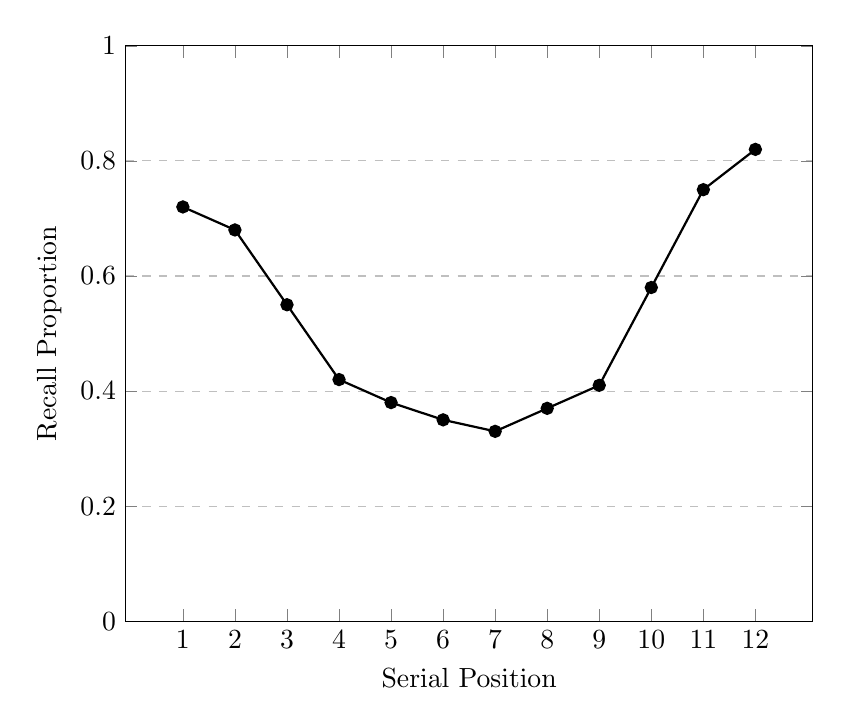
\begin{tikzpicture}
    \begin{axis}[
      width  = 0.85\linewidth,
      xlabel = {Serial Position},
      ylabel = {Recall Proportion},
      xtick  = {1,2,...,12},
      ymin   = 0, ymax = 1,
      ymajorgrids = true,
      grid style  = dashed,
    ]
      \addplot[mark=*, thick] coordinates {
        (1,.72)(2,.68)(3,.55)(4,.42)(5,.38)(6,.35)
        (7,.33)(8,.37)(9,.41)(10,.58)(11,.75)(12,.82)
      };
    \end{axis}
  \end{tikzpicture}
  \caption{Simulated serial position curve ($N = 30$, error bars omitted).
    \textit{Note}. Data are invented for illustrative purposes.}
  \label{fig:spe}
\end{figure}

\begin{figure}[htbp]
  % \includesubgraphics inserts labelled subfigures without sub-captions.
  % Replace example-image-a/b with actual figure files in real use.
  \includesubgraphics{A}{example-image-a}
  \includesubgraphics{B}{example-image-b}
  \caption{Two-panel figure produced with \texttt{\textbackslash
    includesubgraphics}. Panel~A: primacy region (positions 1--3).
    Panel~B: recency region (positions 10--12). \textit{Note}. Placeholder
    images shown; replace with real figures.}
  \label{fig:panels}
\end{figure}

\draftsection{Effect of Presentation Rate}

This section will discuss how varying the inter-stimulus interval modulates
the magnitude of the primacy effect. Data collection for a follow-up
experiment is ongoing.

\section{Discussion}

The simulated data reproduce the classic U-shaped serial position curve,
consistent with \cites{AtkinsonShiffrin1968} dual-store account. Both primacy
and recency were large (Cohen's $d > 0.75$), in line with typical
effect sizes reported in the literature \citeeg{Murdock1962}.

% \colorize marks passages revised in response to reviewer comments.
% Use nocolorize when submitting the clean version.
\colorize{We agree with Reviewer~2 that the implications for
working-memory capacity limits deserve further discussion, and have
expanded this paragraph accordingly.}

\draftsubsection{Comparison With Delayed Recall}

\cites{GlanzerCunitz1966} findings predict that a filled delay should
selectively reduce recency. A direct comparison of immediate and delayed
conditions is planned for future work.

\draftsubsubsection{Potential Confounds}

Word frequency and imageability should be matched across serial positions in
future studies to rule out item-level confounds.
\colorize{Per Reviewer~1: add analysis of frequency effects here.}


% --- Bibliography (inline BBL; no bibtex run needed) ---
% These three papers are real; the data above are not.

\begin{thebibliography}{}

\bibitem [\protect \citeauthoryear {%
Atkinson\ \BBA {} Shiffrin%
}{%
Atkinson\ \BBA {} Shiffrin%
}{%
{\protect \APACyear {1968}}%
}]{%
AtkinsonShiffrin1968}
\APACinsertmetastar {%
AtkinsonShiffrin1968}%
\begin{APACrefauthors}%
Atkinson, R\BPBI C.\BCBT {}\ \BBA {} Shiffrin, R\BPBI M.%
\end{APACrefauthors}%
\unskip\
\newblock
\APACrefYearMonthDay{1968}{}{}.
\newblock
{\BBOQ}\APACrefatitle {Human memory: {A} proposed system and its control
  processes} {Human memory: {A} proposed system and its control
  processes}.{\BBCQ}
\newblock
\APACjournalVolNumPages{The Psychology of Learning and Motivation}{2}{}{89--195}.
\PrintBackRefs{\CurrentBib}

\bibitem [\protect \citeauthoryear {%
Glanzer\ \BBA {} Cunitz%
}{%
Glanzer\ \BBA {} Cunitz%
}{%
{\protect \APACyear {1966}}%
}]{%
GlanzerCunitz1966}
\APACinsertmetastar {%
GlanzerCunitz1966}%
\begin{APACrefauthors}%
Glanzer, M.\BCBT {}\ \BBA {} Cunitz, A\BPBI R.%
\end{APACrefauthors}%
\unskip\
\newblock
\APACrefYearMonthDay{1966}{}{}.
\newblock
{\BBOQ}\APACrefatitle {Two storage mechanisms in free recall} {Two storage
  mechanisms in free recall}.{\BBCQ}
\newblock
\APACjournalVolNumPages{Journal of Verbal Learning and Verbal Behavior}{5}{}{351--360}.
\PrintBackRefs{\CurrentBib}

\bibitem [\protect \citeauthoryear {%
Murdock%
}{%
Murdock%
}{%
{\protect \APACyear {1962}}%
}]{%
Murdock1962}
\APACinsertmetastar {%
Murdock1962}%
\begin{APACrefauthors}%
Murdock, B\BPBI B.%
\end{APACrefauthors}%
\unskip\
\newblock
\APACrefYearMonthDay{1962}{}{}.
\newblock
{\BBOQ}\APACrefatitle {The serial position effect of free recall} {The serial
  position effect of free recall}.{\BBCQ}
\newblock
\APACjournalVolNumPages{Journal of Experimental Psychology}{64}{}{482--488}.
\PrintBackRefs{\CurrentBib}

\end{thebibliography}


% ---------------------------------------------------------------
% Supplementary Materials
% \appendixname is already set to "Supplementary Materials" above,
% so \appendixshortname expands to "SM".
% \myappendix resets page/section/figure/table numbering and,
% because appendixtoc is active, prints a local TOC.
% ---------------------------------------------------------------

\myappendix

% \appsection handles the first section without a preceding page break.
% \appsectionFirst is a deprecated alias kept for backward compatibility;
% use \appsection throughout.
\appsection{Raw Data}

Table~\ref{tab:rawdata} presents the simulated mean recall proportions
by serial position.

\begin{table}[htbp]
  \centering
  \caption{Simulated Mean Recall Proportions by Serial Position}
  \label{tab:rawdata}
  \begin{tabular}{ccc}
    \toprule
    Position & \M  & \SD \\
    \midrule
     1        & .72 & .17 \\
     2        & .68 & .18 \\
     3        & .55 & .16 \\
     4        & .42 & .15 \\
     5        & .38 & .14 \\
     6        & .35 & .14 \\
     7        & .33 & .15 \\
     8        & .37 & .15 \\
     9        & .41 & .16 \\
    10        & .58 & .17 \\
    11        & .75 & .16 \\
    12        & .82 & .15 \\
    \bottomrule
  \end{tabular}
  \par\smallskip
  \textit{Note}. All data are simulated for illustrative purposes.
\end{table}

\appsection{Alternative Analyses}

\subsection{Non-Parametric Tests}

\draftsubsubsection{Confirm wording with statistician}

As a robustness check, we replicated the primacy and recency contrasts
using non-parametric tests. The Wilcoxon signed-rank test confirmed the
primacy effect: \W{}(30) = 412, \Z{} = 3.42, \p{} < .001. The
Mann--Whitney test confirmed the recency advantage: \U{} = 156,
\Z{} = 4.11, \p{} < .001. The standard error of the position-1 recall
proportion was \SE{} = .031. For completeness, the effect-size estimates
were \et{} = .21 (eta-squared) and \etp{} = .23 (partial eta-squared)
from the parametric ANOVA reported in the main text.

\end{document}
